\documentclass[conference]{IEEEtran}
\IEEEoverridecommandlockouts

\usepackage{cite}
\usepackage{amsmath,amssymb,amsfonts}
\usepackage{graphicx}
\usepackage{textcomp}
\usepackage{xcolor}
\usepackage{booktabs}
\usepackage{array}
\usepackage{multirow}
\usepackage{tikz}
\usetikzlibrary{shapes.geometric,arrows.meta,positioning,calc}
\usepackage[hidelinks]{hyperref}
\usepackage{url}
\graphicspath{{figs/}}

\begin{document}

\title{8 Bit Deep Learning Accelerator for
\\GAN Image Generation on GF180MCU}

\author{%
\setlength{\tabcolsep}{0pt}%
\begin{tabular}{@{}>{\centering\arraybackslash}p{0.31\textwidth}
                >{\centering\arraybackslash}p{0.31\textwidth}
                >{\centering\arraybackslash}p{0.31\textwidth}@{}}
\shortstack[c]{William Anthony\\
\textit{Bandung Institute of Technology}\\
13223048\\
Bandung, Indonesia\\
13223048@mahasiswa.itb.ac.id}
&
\shortstack[c]{I Made Medika Surya W.M.\\
\textit{Bandung Institute of Technology}\\
13222021\\
Bandung, Indonesia\\
13222021@mahasiswa.itb.ac.id}
&
\shortstack[c]{John Ruben Saragi\\
\textit{Bandung Institute of Technology}\\
13222049\\
Bandung, Indonesia\\
13222049@mahasiswa.itb.ac.id}
\end{tabular}\\[1.25em]
\begin{tabular}{@{}>{\centering\arraybackslash}p{0.42\textwidth}
                >{\centering\arraybackslash}p{0.42\textwidth}@{}}
\shortstack[c]{Mahardhika Putra Adipratama\\
\textit{Bandung Institute of Technology}\\
13222081\\
Bandung, Indonesia\\
13222081@mahasiswa.itb.ac.id}
&
\shortstack[c]{Fairuz Apuilla Rahagi\\
\textit{Bandung Institute of Technology}\\
13222107\\
Bandung, Indonesia\\
13222107@mahasiswa.itb.ac.id}
\end{tabular}%
}

\maketitle

\begin{abstract}
This paper presents 8 Bit Deep Learning Accelerator for a small GAN image generator on the open GF180MCU 180 nm process. The target network is a three layer multi layer perceptron generator trained on MNIST. The software model is quantized from FP32 to signed 8 bit integers and mapped to a structural $4\times4$ Processing Element array. Each element performs signed multiplication and 24 bit accumulation for tiled matrix multiplication. The A, B, and C operand buffers use eleven physical $256\times8$ SRAM macros instead of inferred register arrays. Verification is done against Python vectors for one matrix multiplication, one layer row, and a full 784 pixel image. The design is implemented with LibreLane on GF180MCU and produces a routed GDS layout with zero Magic DRC errors, zero Netgen LVS errors, and zero antenna violations. The final layout uses a $1.6\times1.5$ mm$^2$ die and meets a 75 ns clock across the evaluated STA corners.
\end{abstract}

\begin{IEEEkeywords}
Deep Learning Accelerator, GF180MCU, SRAM macro, systolic array, INT8 quantization, GAN, ASIC, LibreLane.
\end{IEEEkeywords}

\section{Introduction}
Generative Adversarial Networks can be used as a compact workload for testing neural inference on custom hardware. In this work, the generator is a small MNIST multi layer perceptron that converts a 64 dimensional latent vector into a $28\times28$ image. The arithmetic is mostly dense matrix multiplication, so the workload can be mapped to a small systolic array.

The naive design using sequential behavioral loops and memory arrays in Verilog was easier to simulate because it used sequential behavioral loops and memory arrays in Verilog. That version was useful for checking the algorithm, but was not suitable for the ASIC implementation. If the model weights and buffers are inferred as standard cell registers, the design becomes too large and difficult to route. For this reason, the design was changed into a structural accelerator with a Processing Element array, local SRAM backed buffers, and a small controller.

\section{Related Work}
Most neural network accelerators are built around arrays of multiply and accumulate units. A well known large scale example is the systolic Tensor Processing Unit \cite{tpu}, and a broad overview of deep learning accelerators for different platforms is given in \cite{survey}. To run a floating point network on this kind of integer array, the weights and activations are usually quantized with a per tensor scale, as described by Jacob et al. \cite{jacob}.

The closest work to ours is Wang et al. \cite{wang}, which presents a small PE array accelerator for an underwater recognition network in a 40 nm process. Our design is different because it targets the open GF180MCU 180 nm process and uses a full open source flow from RTL to GDS. The workload is a pretrained MLP GAN \cite{goodfellow, ganpretrained}, and the RTL is based on the open DLA Engine project \cite{dlaengine}.

\section{GAN Architecture}\label{sec:overview}

The GAN generator architecture uses a multi-layer perceptron (MLP) model that receives a latent vector of size 64 as the initial input. This input is then projected through two hidden layers, each containing 256 neurons, to form a richer feature representation. Each hidden layer is followed by a ReLU activation function, allowing the model to learn non-linear patterns from the data.

\begin{figure}[h]
\centering
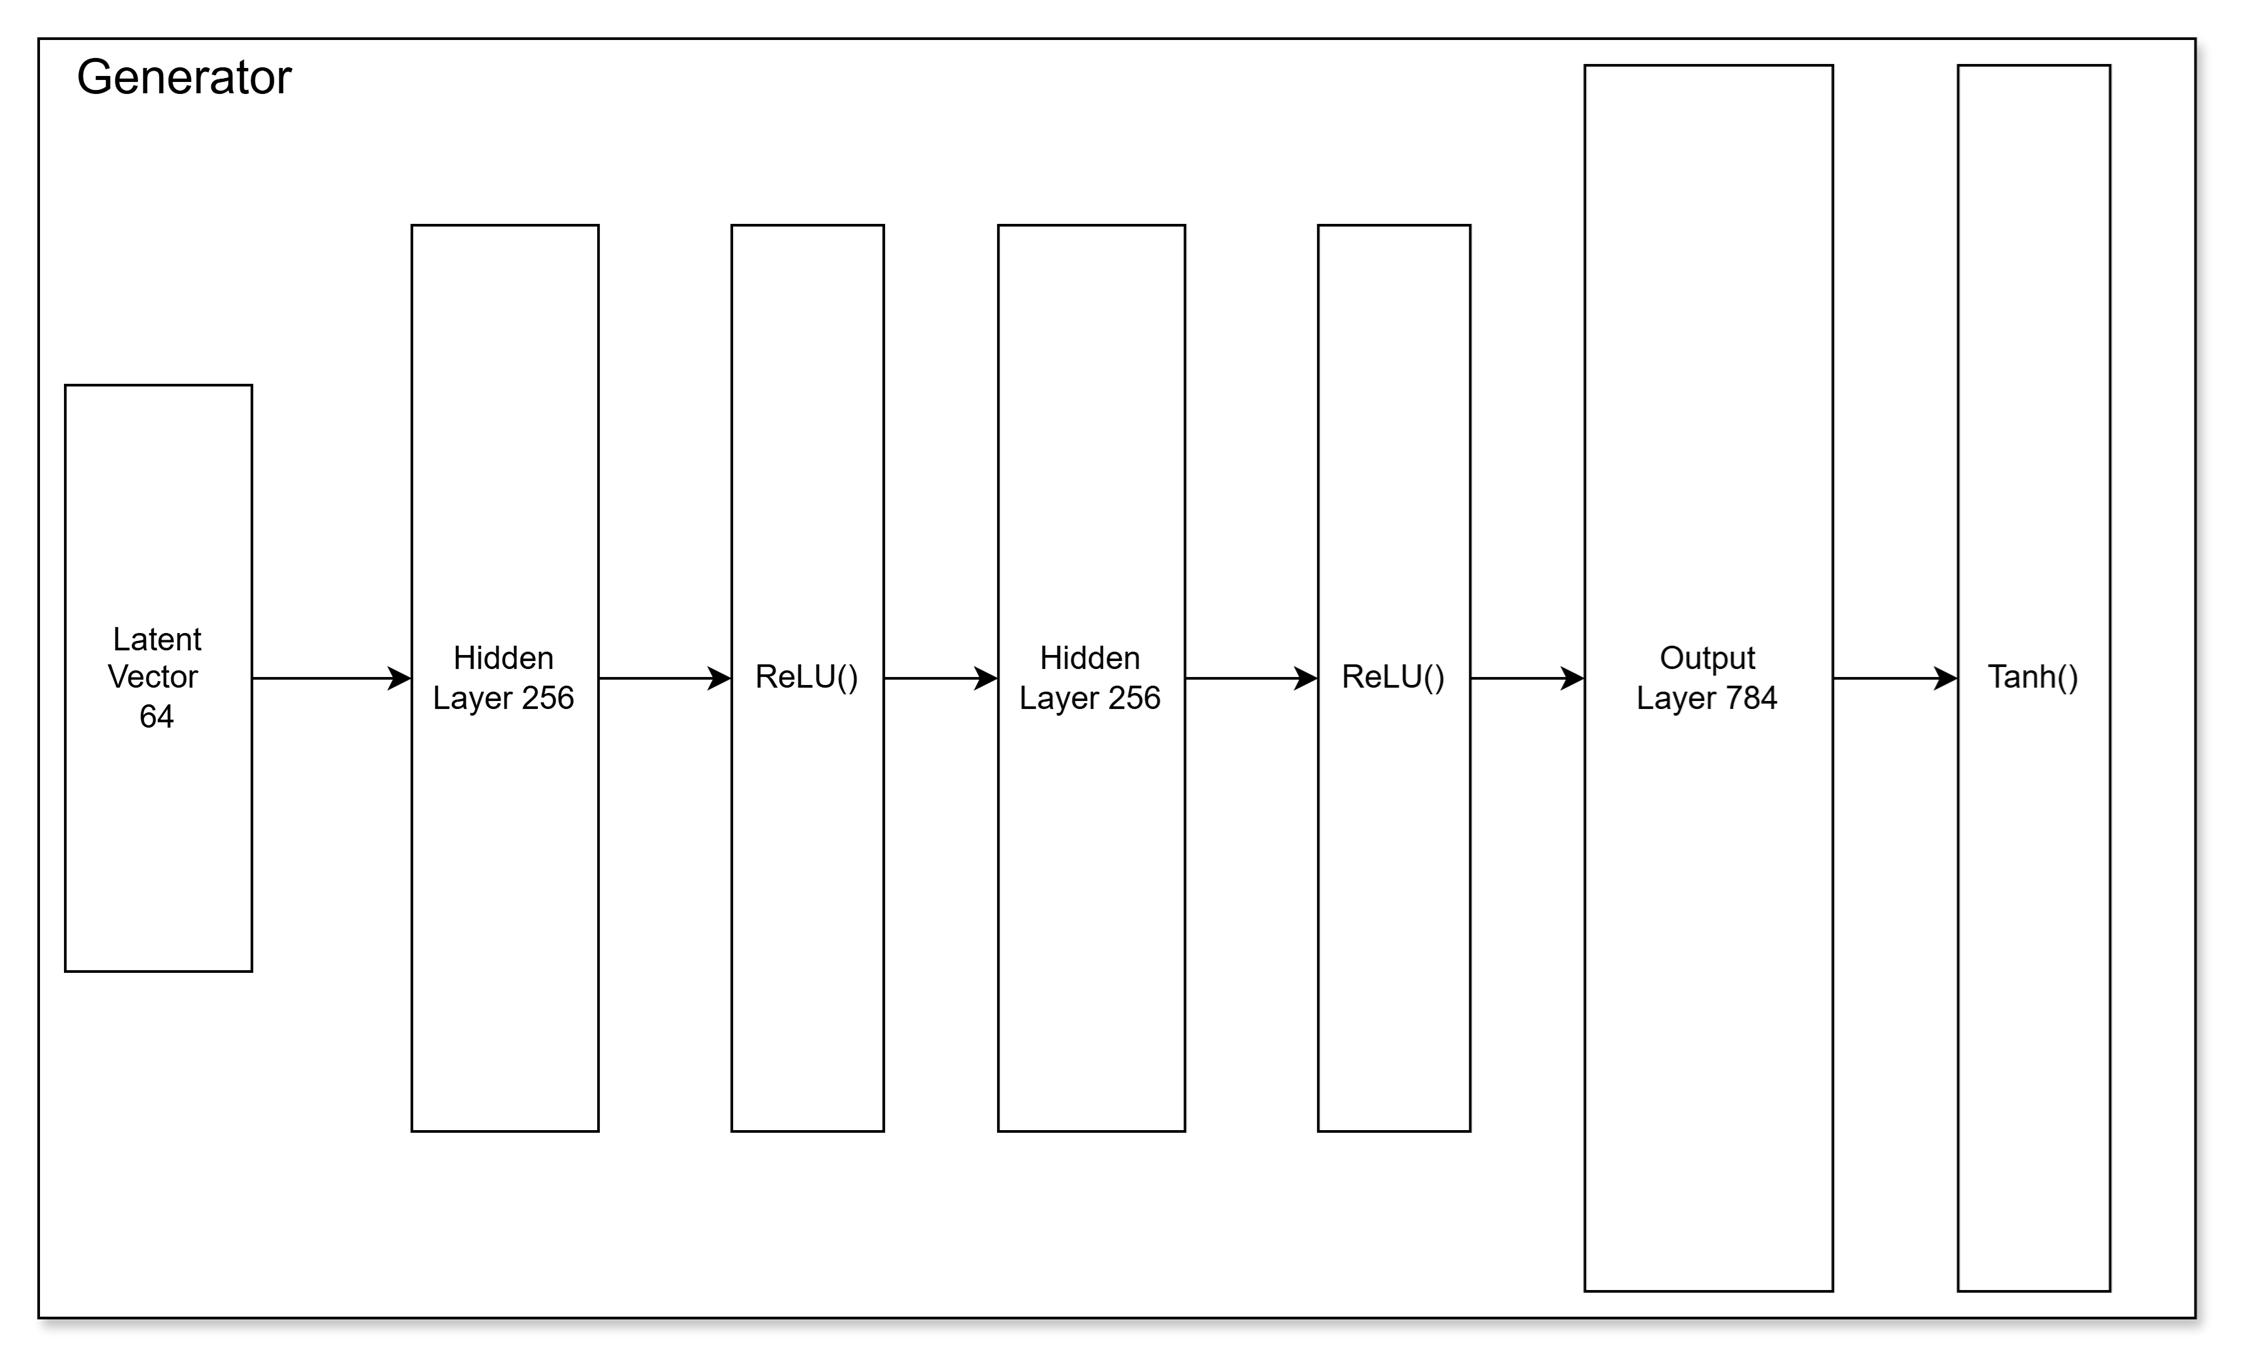
\includegraphics[width=\columnwidth]{figs/GAN_Generator_layers.png}
\caption{GAN Generator Layer Architecture}
\label{fig:top}
\end{figure}

After that, the learned representation is passed to an output layer with 784 neurons, which corresponds to a 28 × 28 pixel image. In the final stage, a Tanh activation function is used to limit the output values to a certain range, usually between -1 and 1, so that the output of the generator can be represented as a grayscale image. Through this process, the generator transforms a random vector into a synthetic image that resembles real data.

Table \ref{tab:net} lists the three dense layers and shows how many tiles each layer needs on the $4\times4$ array. Because the array produces four output values per tile, the layer with 784 outputs needs the most tiles.

\begin{table}[h]
\caption{Generator layers and their mapping to the $4\times4$ array.}
\label{tab:net}
\centering
\renewcommand{\arraystretch}{1.15}
\begin{tabular}{@{}lcccc@{}}
\toprule
Layer & Output $\times$ Input & Activation & Tiles & MAC ops \\
\midrule
L0 & $256\times64$  & ReLU & 64  & 16{,}384  \\
L2 & $256\times256$ & ReLU & 64  & 65{,}536  \\
L4 & $784\times256$ & Tanh & 196 & 200{,}704 \\
\midrule
Total & & & 324 & 282{,}624 \\
\bottomrule
\end{tabular}
\end{table}

\section{Hardware Architecture}\label{sec:hw}

The DLA computes a tiled matrix multiplication $C=A\times B$. The default array size is $N=4$, and the inner dimension used for the generator layers is $K=256$. During one transaction, the controller clears the PE accumulators, enables the array for $K$ cycles, then stores the result block to the C buffer.

\begin{figure}[h]
\centering
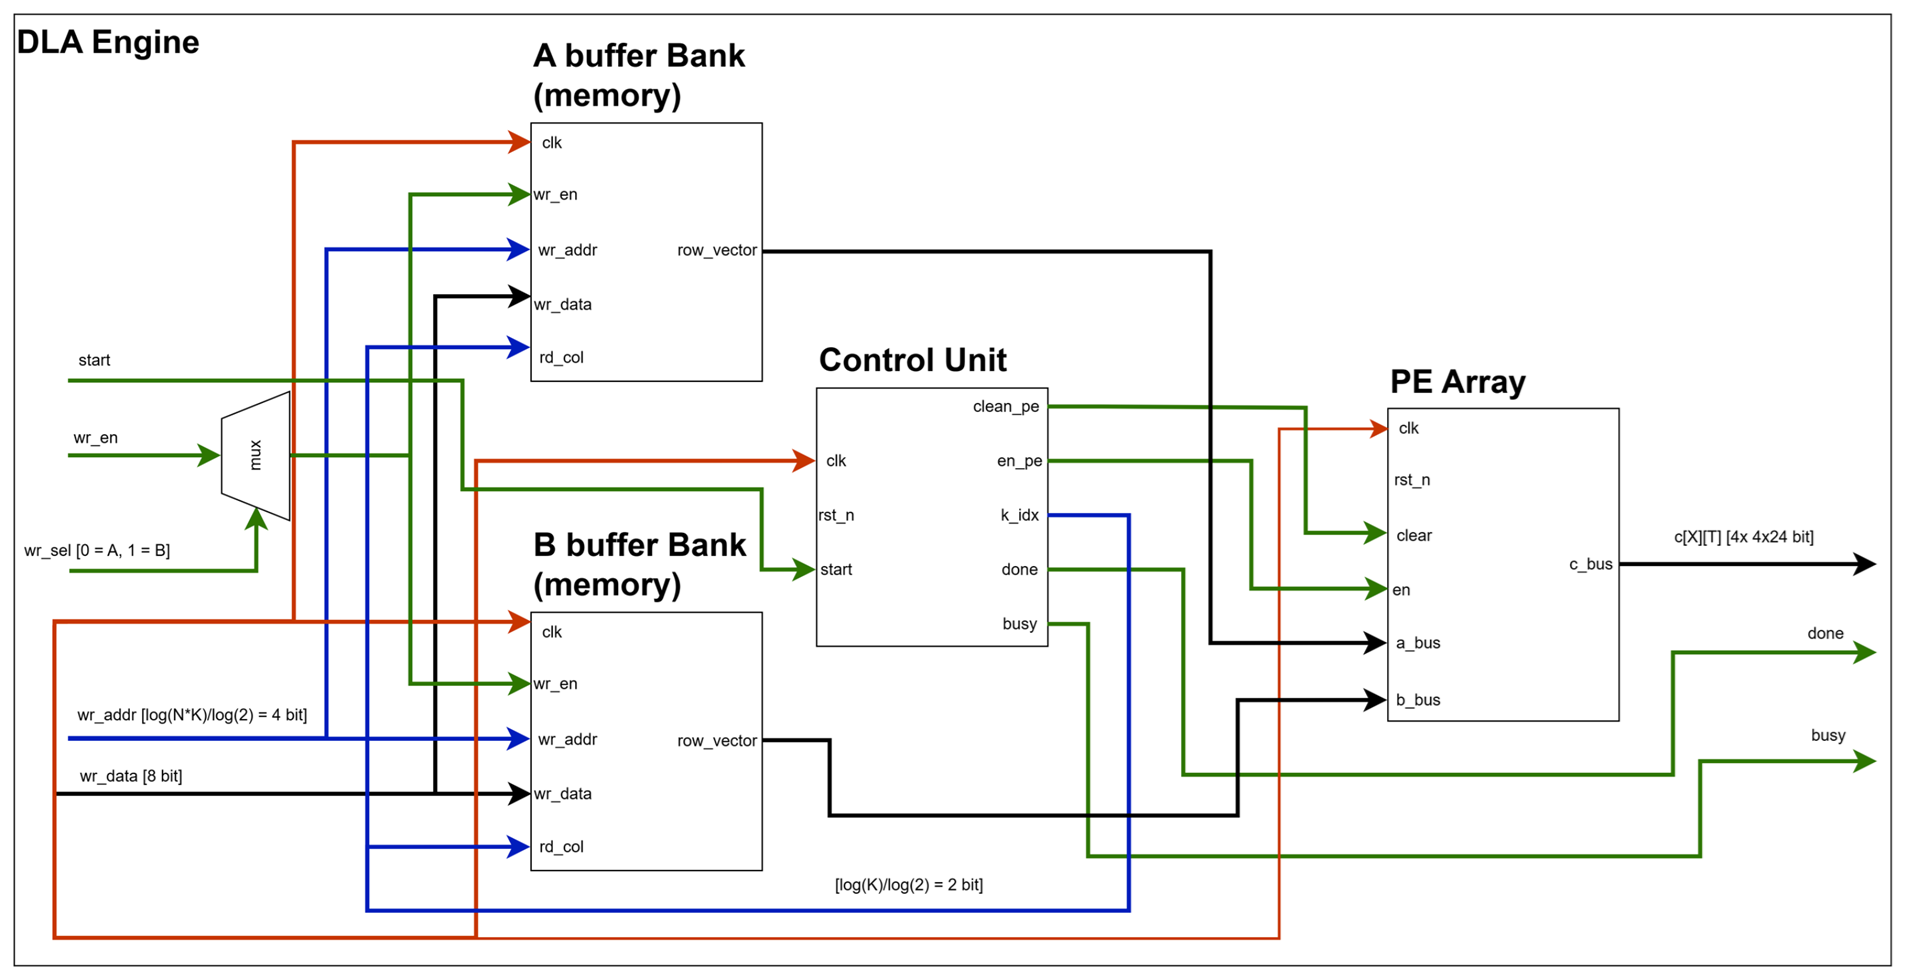
\includegraphics[width=\columnwidth]{Top_level.png}
\caption{DLA Engine Top Level}
\label{fig:top}
\end{figure}

The Top Level consist of A buffer provides one row vector to the PE array, and the B buffer provides one column vector. The control unit generates the read index, clear signal, enable signal, done signal, and busy signal. The output bus carries the accumulated C values.

\subsection{Processing Element}

Each Processing Element receives two signed 8 bit inputs. It multiplies them, sign extends the 16 bit product to 24 bits, and adds it to a local accumulator. The accumulator is reset  and cleared at the start of each matrix multiplication. The output of each PE is one partial dot product.

\begin{figure}[h]
\centering
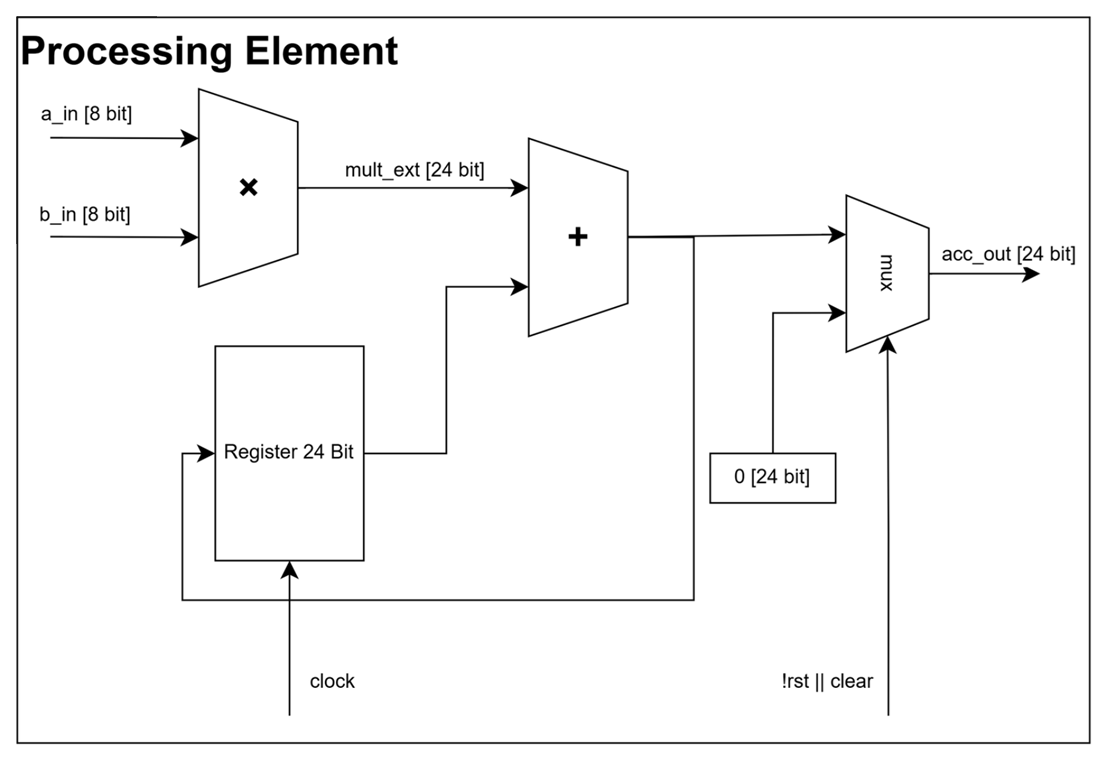
\includegraphics[width=0.8\columnwidth]{PE.png}
\caption{Processing element datapath.}
\label{fig:pe}
\end{figure}

The main computation in one PE follows
\begin{equation}
acc_{out}[n] = acc_{out}[n-1] + a_{in}[n]b_{in}[n].
\end{equation}
After $K$ cycles, the accumulator stores one output value of the matrix multiplication tile. A 24 bit accumulator is used so that the sum of 8 bit products has enough range for the selected layer sizes.

\subsection{PE Array}
The PE array instantiates 16 PEs in a $4\times4$ grid. Each row receives one activation lane, and each column receives one weight lane. All 16 PEs operate in parallel, so the array produces one $4\times4$ output tile after the accumulation loop finishes.

The $a\_bus$ contains four 8 bit activation values, while the $b\_bus$ contains four 8 bit weight values. The output $c\_bus$ is flattened from 16 accumulator outputs, each with 24 bits.

\begin{figure}[h]
\centering
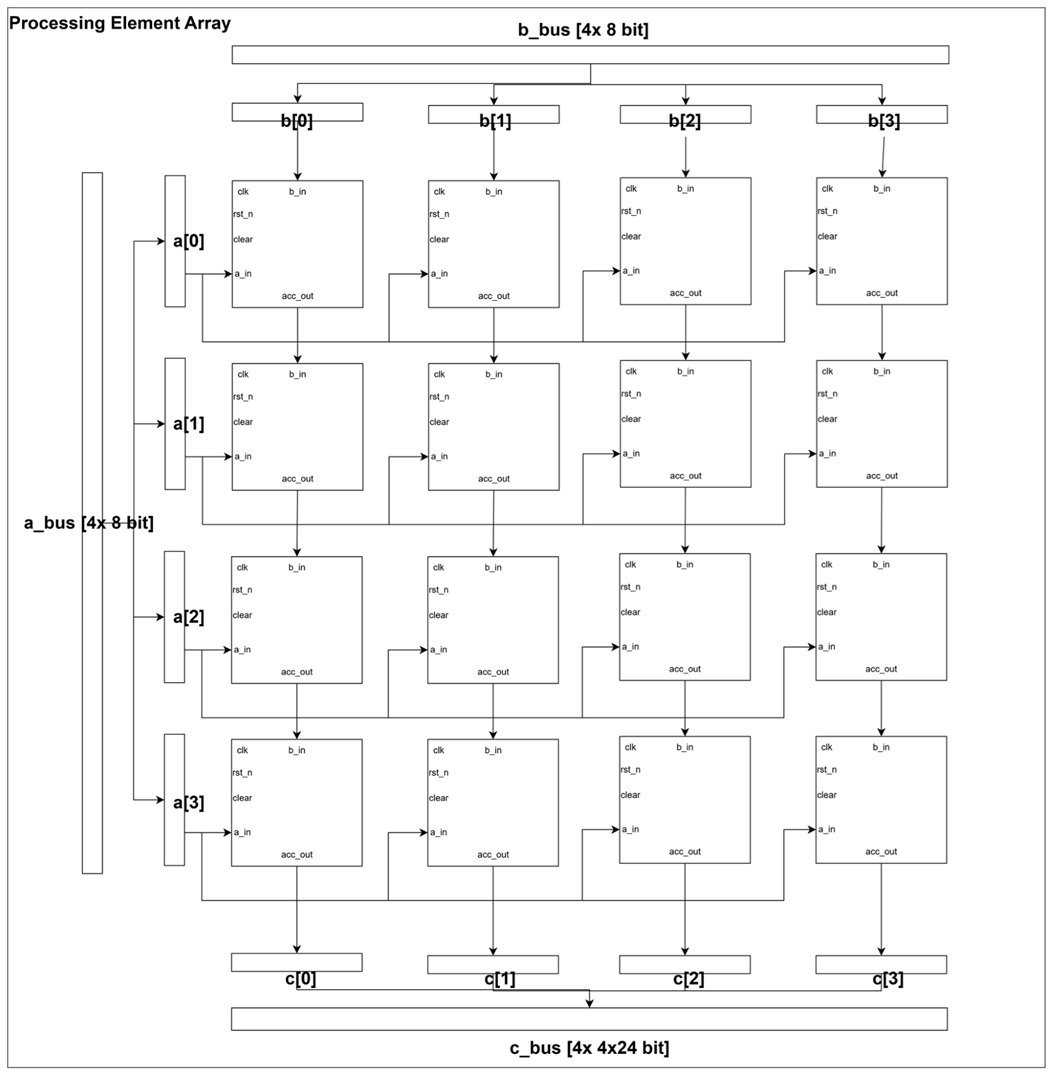
\includegraphics[width=\columnwidth]{PE_Array.png}
\caption{Processing element array.}
\label{fig:pearray}
\end{figure}

\subsection{Controller FSM}
The controller uses four states. In IDLE, it waits for START. In CLEAR, it clears all PE accumulators for one cycle. In COMPUTE, it asserts ENABLE PE ARRAY and increments the buffer A and B memory address until all $K$ address terms have been processed. In DONE, it raises DONE and waits for START to return low before going back to IDLE.

\begin{figure}[h]
\centering
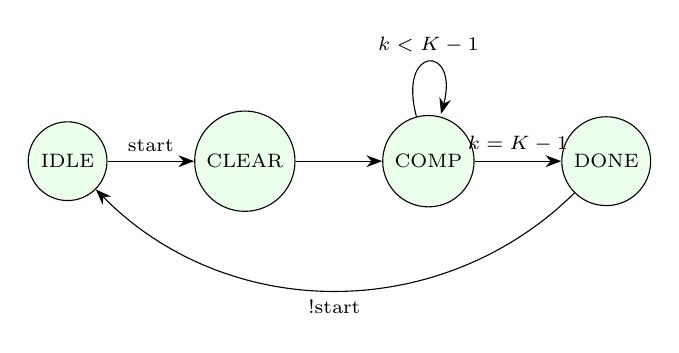
\begin{tikzpicture}[
  font=\scriptsize,>={Stealth[length=2mm]},
  st/.style={draw,circle,minimum size=10mm,fill=green!8}
]
\node[st] (idle) {IDLE};
\node[st,right=11mm of idle] (clear) {CLEAR};
\node[st,right=11mm of clear] (comp) {COMP};
\node[st,right=11mm of comp] (done) {DONE};
\draw[->] (idle) -- node[above]{start} (clear);
\draw[->] (clear) -- (comp);
\path (comp) edge[->,loop above] node{$k<K-1$} (comp);
\draw[->] (comp) -- node[above]{$k=K-1$} (done);
\draw[->] (done) to[bend left=45] node[below]{!start} (idle);
\end{tikzpicture}
\caption{Controller state machine.}
\label{fig:fsm}
\end{figure}

\subsection{SRAM Buffers}
The input and output buffers are implemented with physical $256\times8$ single port SRAM macros. The A buffer uses four macros, one for each row lane. The B buffer also uses four macros, one for each column lane. The C buffer stores 24 bit accumulator outputs by using three 8 bit SRAM macros. In total, the design uses eleven SRAM macros.

The SRAM wrapper has a behavioral memory model for simulation and a synthesis branch for the hard macro. In simulation, the memory is represented by a Verilog register array so that the testbench can run normally. During synthesis, the memory is treated as a macro blackbox. The power pins are not tied to logic constants in RTL. They are connected by the physical power delivery network during place and route.

The SRAM read has one cycle of latency. Because of that, the top level delays the PE enable and completion flags by one cycle so that the data and control signals stay aligned. This keeps the PE array from accumulating invalid data after a read request.

\section{Software to Hardware Flow}\label{sec:sw}

The system is separated into the hardware core and the verification environment. The hardware core is The DLA Top Engine. It contains the A and B input buffers, the C output buffer, the controller, and the $4\times4$ PE array. This is the part that is synthesized and routed. The verification environment is written in Python and Verilog. It prepares quantized weights, input vectors, and reference outputs, then drives the accelerator through its normal read and write ports.

\begin{figure}[h]
\centering
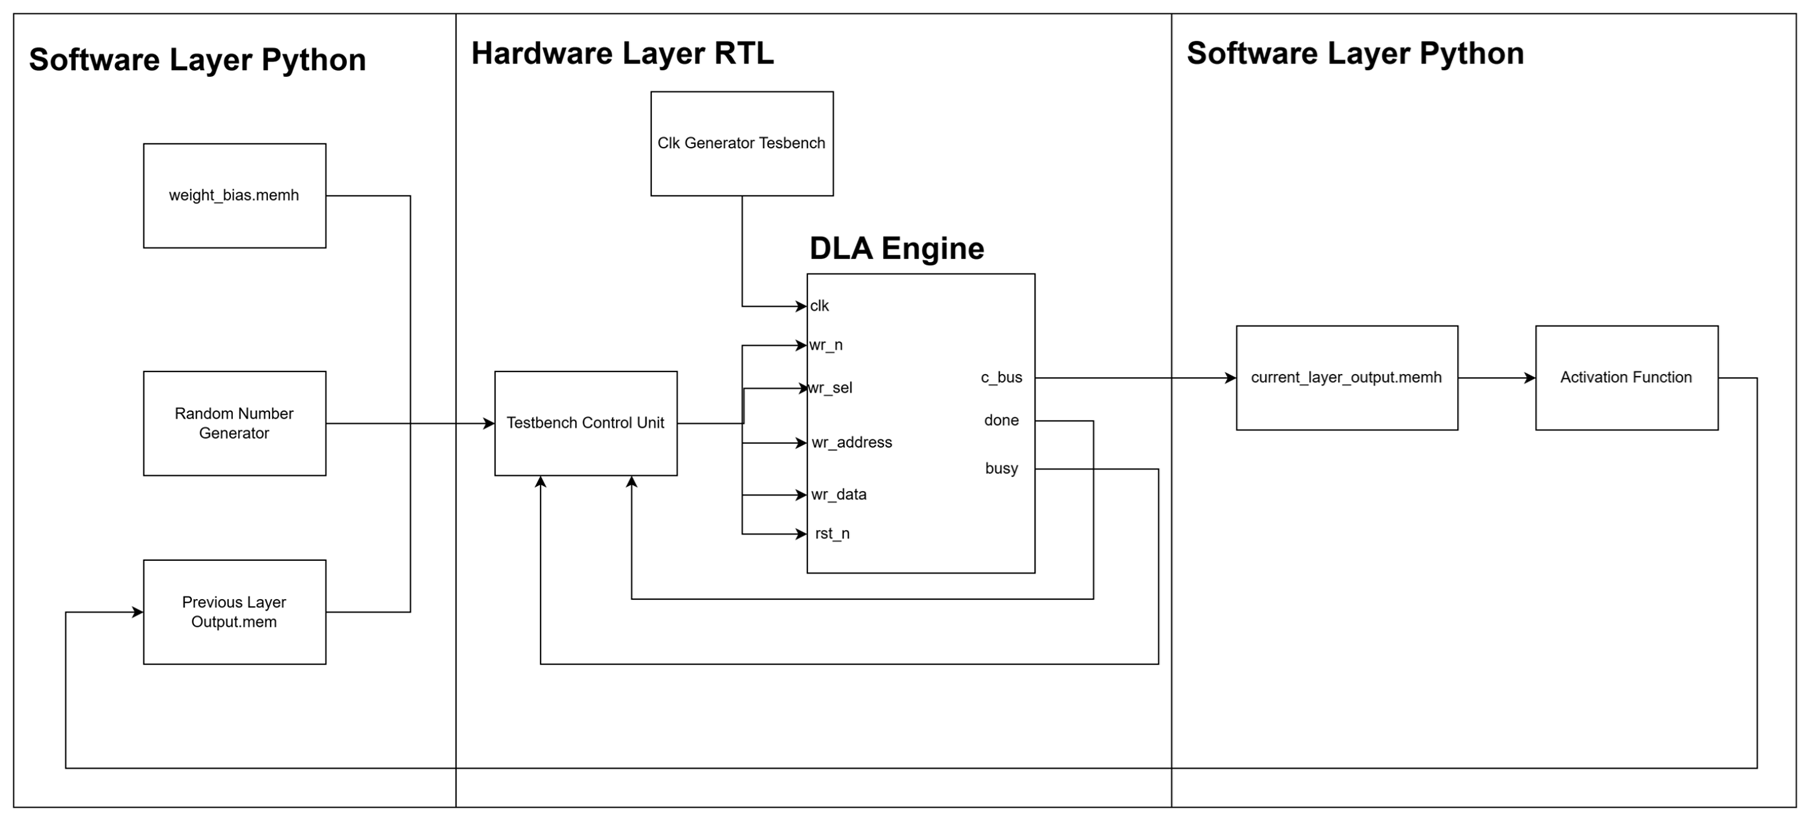
\includegraphics[width=0.8\columnwidth]{Hardware_Software_Integration.png}
\caption{Hardware and Software Flow}
\label{fig:hwsoft}
\end{figure}

Python prepares the input data and memory contents, then the RTL testbench loads the data to the hardware engine. After the engine finishes, the output is read back and passed to the activation function stage. This split keeps the accelerator simple, while still allowing the complete GAN pipeline to be checked.

\subsection{Quantization and Requantization}
The original model weights are stored as 32 bit floating point values. Before they can be used by the integer array, every weight and bias tensor is converted to signed 8 bit values using one scale factor per tensor. The scale comes from the largest absolute value in the tensor, and all scales are saved in a manifest file so the testbench can reuse the same values.

The DLA only returns the integer dot product of one tile. The rest of the math is done around it in integer form, so the hardware result matches the Python reference. For the two hidden layers, the integer result is rescaled, the bias is added, and a ReLU activation is applied before the value is quantized again to 8 bits for the next layer. For the output layer, the result is turned into a fixed point value, passed through a tanh lookup table, and then mapped to a grayscale pixel. The lookup table is used so that tanh does not have to be computed directly in hardware.

\section{RTL Verification}\label{sec:map}

To verify the GAN RTL result, the generator is mapped to the DLA as a sequence of tiled dense layers. For each tile, four output neurons are computed at the same time. They four weight rows are written to the A buffer bank, and the shared input vector is written into the B buffer. The DLA then performs the dot products and stores the four selected results in the C buffer.

\begin{table}[h]
\caption{Verification results.}
\label{tab:verif}
\centering
\renewcommand{\arraystretch}{1.15}
\begin{tabular}{@{}lll@{}}
\toprule
Testbench & Check & Result \\
\midrule
\texttt{d3004\_tb} & one GEMM & PASS \\
\texttt{g3005\_tb} & one layer row & PASS \\
\texttt{g300\_pipeline\_tb} & full image & PASS \\
\bottomrule
\end{tabular}
\end{table}

Layer L0 uses the 64 dimensional latent vector as input. Layer L2 uses the 256 dimensional activation from L0. Layer L4 also uses a 256 dimensional input and produces 784 pixel values. Since the array has four output lanes, L0 and L2 each require 64 tiles, while L4 requires 196 tiles. The same DLA datapath is reused for all layers.

\begin{figure}[h]
\centering

\includegraphics[width=0.22\linewidth]{digit_seed6.jpg}\hspace{4mm}

\includegraphics[width=0.22\linewidth]{digit_seed5.jpg}\hspace{4mm}

\includegraphics[width=0.22\linewidth]{digit_seed9.jpg}
\caption{Generated Digit Samples}
\label{fig:samples}
\end{figure}

The pictures Shows examples of generated $28\times28$ images. The visual quality is limited by the small generator and by INT8 quantization, but the images are enough to verify that the full software to hardware path is running.

\section{Physical Implementation}\label{sec:phys}

The design is implemented with LibreLane on the GF180MCU process. The standard cell library GF018HV5V, while the external SRAM macro used for the buffers is GF180MCU OCD ID SRAM $256\times8\times8$ wm. The eleven SRAM macros are placed manually on a grid with routing channels between them. The final standard cell count is much smaller than the register memory version because the buffers are implemented as hard macros.

\begin{figure}[h]
\centering
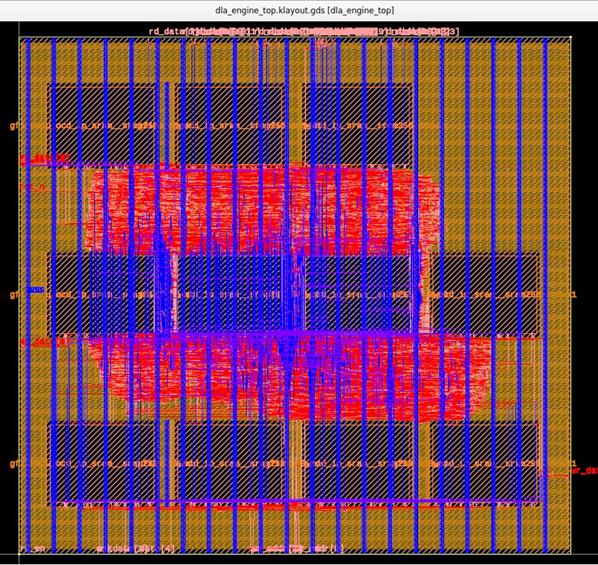
\includegraphics[width=0.8\columnwidth]{Final_GDS.png}
\caption{Final GDS Layout}
\label{fig:layout}
\end{figure}

Several practical issues appeared during physical implementation. The SRAM power pins had to be left as physical macro pins instead of being tied in RTL. The macro LEF, GDS, and Liberty files had to be registered in the flow, and each macro instance had to be placed explicitly. The die was set to $1600\times1500~\mu$m to fit the eleven SRAM macros and the surrounding logic. A small amount of standard cell padding was also needed to improve detailed placement and diode access.

The power grid also needed a change. The SRAM power pins only reach Metal3, so the macro power connection had to be made on Metal3 instead of the default higher layers, otherwise the power network did not connect. Routing was allowed up to Metal5 so the tool had more room to fix antenna problems on long nets. One more important setting is the synthesis define that keeps the SRAM as a hard macro. Without it, the memory is built from flip flops and no macro appears in the layout.

The antenna check required multiple layout iterations. Direct in router antenna repair did not finish reliably because some rerouted nets failed pin access. Larger floorplan changes also did not help, because they tended to create new long routes. The final clean run was obtained by keeping the macro grid and changing the placement density target from 55 percent to 56 percent. This small change altered the routing enough to remove the last antenna violation while keeping timing, DRC, and LVS clean.

Table \ref{tab:antenna} shows the antenna result for the layout runs that finished. The in router jumper repair could not be used here, because the repair step tried to reroute nets that had no pin access and the run stopped with a routing error. Adding more protection diodes did not help either, because the last net already had several diodes and still failed, so the real problem was the wire length and not the number of diodes. Every large floorplan change, such as clustering the macros or packing them tighter, made the antenna count worse instead of better. The clean result came from the small density change on the same grid. Because the flow is deterministic, running the final configuration again gave a layout with the same zero antenna result.

\begin{table}[h]
\caption{Antenna result across the layout runs that finished.}
\label{tab:antenna}
\centering
\renewcommand{\arraystretch}{1.15}
\begin{tabular}{@{}lccl@{}}
\toprule
Floorplan change & Antenna nets & Setup slack & Result \\
\midrule
Grid baseline, 75 ns  & 1 & $+9.07$  & one net left \\
Clustered macros      & 4 & $+14.05$ & worse \\
Clustered, density 70 & 3 & $+7.10$  & worse \\
Grid, max fanout 4    & 6 & $-13.78$ & worse, timing failed \\
A row swapped         & 3 & $+9.0$   & worse \\
B row swapped         & 5 & $+10.5$  & worse \\
A and B rows swapped  & 3 & $+14.67$ & worse \\
Grid, density 56      & 0 & $+7.58$  & clean signoff \\
\bottomrule
\end{tabular}
\end{table}

\begin{table}[h]
\caption{Physical results.}
\label{tab:signoff}
\centering
\renewcommand{\arraystretch}{1.15}
\begin{tabular}{@{}ll@{}}
\toprule
Metric & Value \\
\midrule
Process & GF180MCU \\
Die area & $1600\times1500~\mu$m \\
Core area & $2.326$ mm$^2$ \\
Utilization & $48.2\%$ \\
SRAM macros & 11 \\
Standard cells & 32,984 \\
Sequential cells & 400 \\
Clock period & 75 ns \\
Worst setup slack & $+7.58$ ns \\
Worst hold slack & $+0.22$ ns \\
Magic DRC & 0 errors \\
Netgen LVS & 0 errors \\
Antenna & 0 nets, 0 pins \\
Power & 189.6 mW \\
\bottomrule
\end{tabular}
\end{table}

The final implementation passes the main physical checks with Magic reports zero DRC errors, Netgen reports zero LVS errors, and the antenna report has zero violating nets and pins. The design meets a 75 ns clock period. The reported nominal power is 189.6 mW, mostly internal power from the selected standard cell and SRAM implementation.

\begin{table}[h]
\caption{STA slack summary.}
\label{tab:corners}
\centering
\renewcommand{\arraystretch}{1.15}
\begin{tabular}{@{}lccc@{}}
\toprule
 & TT & SS & FF \\
\midrule
Setup slack & $+39.69$ & $+9.47$ & $+52.82$ \\
Hold slack  & $+0.52$  & $+1.19$ & $+0.23$  \\
\bottomrule
\end{tabular}
\end{table}

\subsection{Comparison}
Table \ref{tab:compare} compares this work with a recent accelerator by Wang et al. \cite{wang}. Their design uses a smaller PE array on a 40 nm process and is not built with an open source flow. Our design uses a larger array on the older 180 nm GF180MCU process and is built fully with open tools. The larger area and the higher power mostly come from the coarser process and the conservative clock, not from the architecture. The main advantage of this work is that the whole flow is open and the result can be reproduced.

\begin{table}[h]
\caption{Comparison with a recent accelerator.}
\label{tab:compare}
\centering
\renewcommand{\arraystretch}{1.15}
\begin{tabular}{@{}lcc@{}}
\toprule
Parameter & Wang et al. (2024) & This work \\
\midrule
Technology       & TSMC 40 nm                 & GF180MCU 180 nm \\
Architecture     & $2\times2\times2$ PE array & $4\times4\times4$ PE array \\
Core area        & 11.97 mm$^2$               & 2.326 mm$^2$ \\
Total power      & 96.35 mW                   & 189.6 mW \\
Open source flow & No                         & Yes \\
\bottomrule
\end{tabular}
\end{table}

\section{Discussion}\label{sec:disc}
The accelerator can perform 16 MAC operations per cycle, or about 0.43 GOPS at 13.3 MHz. The end to end generator speed is still limited by loading data into the local buffers. Each tile must load weight rows and the shared input vector before the compute phase. Better weight reuse, streaming, or double buffering would improve the PE utilization. The tests so far use saved vectors, so checking more latent seeds and random inputs would add more confidence in the design.

The implementation also shows a tradeoff between timing and antenna closure. Some floorplans gave better timing slack, but they increased the number of antenna violations. For this version, the priority was a clean physical signoff rather than the fastest possible clock. A later revision can revisit the floorplan if higher throughput is needed.

The current voltage setup should also be treated carefully. The design uses 5 V standard cells, while the SRAM macro is a 3.3 V part. The open GF180MCU PDK only ships a 5 V standard cell library, so the logic cannot be moved to 3.3 V. The present design mixes two voltage domains, which is fine for the layout checks but would need level shifting or a separate supply on real silicon. A planned next step is to swap the buffers to a 5 V SRAM family so the whole design can run from one supply before any chip top integration.

\section{Conclusion}\label{sec:concl}
This architecture implements a small INT8 GAN generator accelerator on GF180MCU. The design replaces behavioral memory arrays with SRAM macros, uses a $4\times4$ PE array for tiled matrix multiplication, and verifies the output against Python reference data. The final LibreLane implementation produces a routed GDS layout with clean DRC, LVS, and antenna reports. The main remaining work is improving data reuse for higher throughput and resolving the voltage domain choice before chip top integration.

\section*{Acknowledgment}
The authors thank the open source EDA community and the GlobalFoundries open shuttle programs for the GF180MCU PDK and the SRAM macro used in this work.

\section*{Author Contributions}
William Anthony worked on the RTL architecture, the PE array design, the RTL to GDS flow, and verification. I Made Medika Surya W.M. worked on the RTL architecture, the MLP GAN architecture, the block diagrams, and verification. John Ruben Saragi worked on the GAN concept, the RTL architecture, and verification. Fairuz Apuilla Rahagi worked on the RTL architecture and the RTL to GDS flow. Mahardhika Putra Adipratama worked on the RTL architecture, verification, and the RTL to GDS flow.

\begin{thebibliography}{9}
\bibitem{ganpretrained} C. Singh, ``GAN/VAE pretrained PyTorch models,'' \url{https://github.com/csinva/gan-vae-pretrained-pytorch}.
\bibitem{gf180sram} R. T. Edwards, ``GF180MCU OCD IP SRAM macros,'' \url{https://github.com/RTimothyEdwards/gf180mcu_ocd_ip_sram}.
\bibitem{librelane} The OpenROAD/LibreLane project, ``LibreLane: an open source RTL to GDSII flow,'' \url{https://github.com/librelane/librelane}.
\bibitem{gf180pdk} GlobalFoundries and Google, ``GF180MCU open source PDK,'' \url{https://github.com/google/gf180mcu-pdk}.
\bibitem{goodfellow} I. Goodfellow, J. Pouget-Abadie, M. Mirza, B. Xu, D. Warde-Farley, S. Ozair, A. Courville, and Y. Bengio, ``Generative adversarial nets,'' in \emph{Proc. NeurIPS}, 2014.
\bibitem{jacob} B. Jacob, S. Kligys, B. Chen, M. Zhu, M. Tang, A. Howard, H. Adam, and D. Kalenichenko, ``Quantization and training of neural networks for efficient integer arithmetic only inference,'' in \emph{Proc. IEEE/CVF CVPR}, 2018.
\bibitem{tpu} N. P. Jouppi \emph{et al.}, ``In datacenter performance analysis of a tensor processing unit,'' in \emph{Proc. ISCA}, 2017.
\bibitem{wang} C. C. Wang, S. H. Luo, H. C. Wu, R. G. B. Sangalang, C. P. Jou, and H. Hsia, ``A 54.61 GOPS 96.35 mW digital logic accelerator for underwater object recognition DNN using 40 nm CMOS process,'' in \emph{Proc. IEEE 6th Int. Conf. AI Circuits and Systems (AICAS)}, 2024.
\bibitem{survey} ``A survey on deep learning hardware accelerators for heterogeneous HPC platforms,'' \emph{ACM Computing Surveys}, 2025.
\bibitem{dlaengine} ``DLA Engine,'' GitHub, \url{https://github.com/wlmoi/DLA_Engine}.
\end{thebibliography}

\end{document}
